\documentclass[10pt]{article}
\usepackage{longtable}
\usepackage{float}
\usepackage{wrapfig}
\usepackage{rotating}
\usepackage[normalem]{ulem}
\usepackage{amsmath}
\usepackage{textcomp}
\usepackage{marvosym}
\usepackage{wasysym}
\usepackage{amssymb}
\usepackage{hyperref}
\usepackage{color,soul} % for highlighting
\usepackage{graphicx}
\graphicspath{{/Users/benjaminbass/seacloud/class/earthMaterials/mineralSheets/tectosilicates/quartz/images/}}

\usepackage{frame,color}
\usepackage{framed}
\usepackage{minibox}

% \usepackage[T1]{fontenc}
% \usepackage{tilting} %bring title up
% \setlength{\droptitle}{-10cm}

\usepackage[version=3]{mhchem}
% How to Use MChem
% \ce{SO4^2-}
% \ce{^{227}_{90}Th+}
% \ce{A\bond{-}B\bond{=}C\bond{#}D}
% \ce{CO2 + C -> 2CO}
% \ce{SO4^2- + Ba^2+ -> BaSO4 v}


\author{Benjamin Bass}
\date{24 February 2016}
\title{\vspace{-2.0cm}Quartz} %bring title up temporary Fix

\begin{document}

\maketitle

% \framebox{Use frameboxes until figure out alignmen}

\begin{center}
  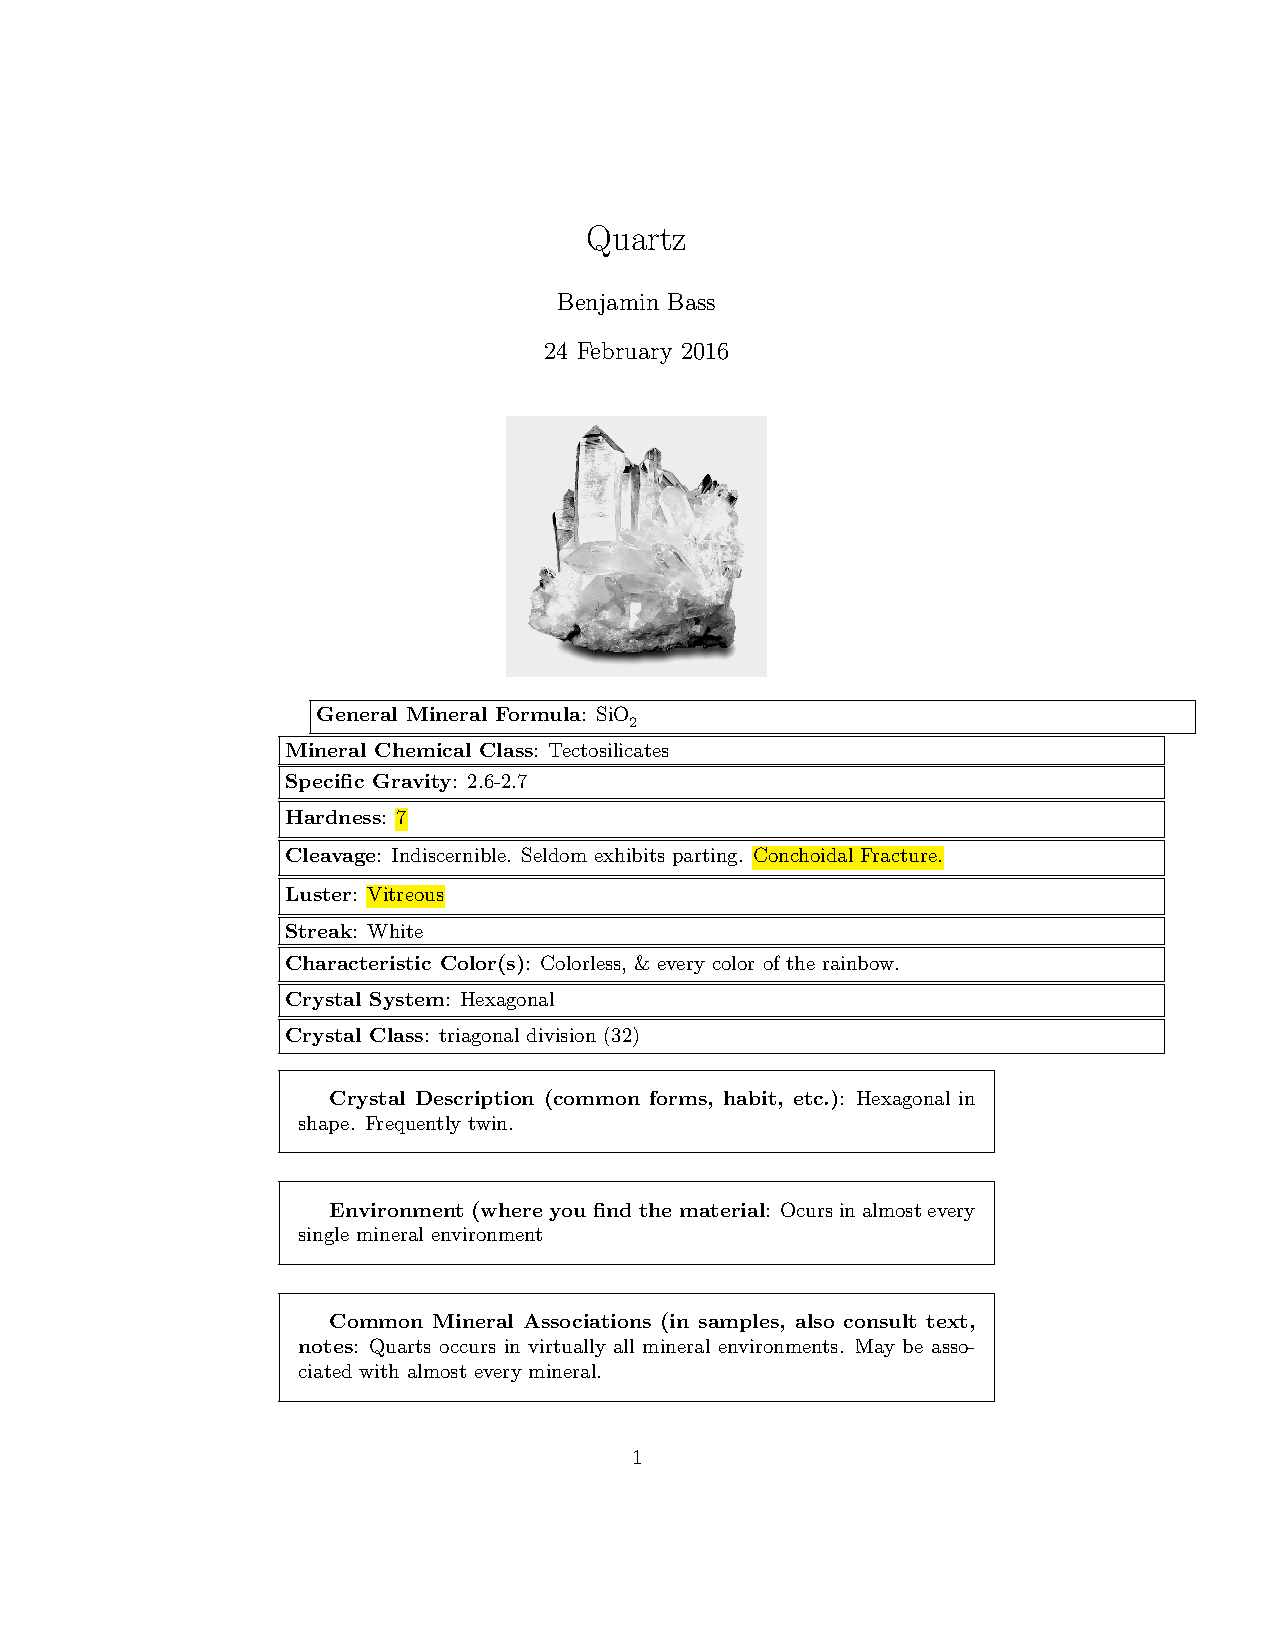
\includegraphics[scale=.25]{quartz}
\end{center}



\framebox[15cm][l]{\textbf{General Mineral Formula}: \ce{SiO2} }\
\framebox[15cm][l]{\textbf{Mineral Chemical Class}: Tectosilicates }\
\framebox[15cm][l]{\textbf{Specific Gravity}: 2.6-2.7 }\
\framebox[15cm][l]{\textbf{Hardness}: \hl{7} }\
\framebox[15cm][l]{\textbf{Cleavage}: Indiscernible. Seldom exhibits parting. \hl{Conchoidal Fracture.} }\
\framebox[15cm][l]{\textbf{Luster}: \hl{Vitreous} }\
\framebox[15cm][l]{\textbf{Streak}: White }\
\framebox[15cm][l]{\textbf{Characteristic Color(s)}: Colorless, \& every color of the rainbow. }\
\framebox[15cm][l]{\textbf{Crystal System}: Hexagonal }\
\framebox[15cm][l]{\textbf{Crystal Class}: triagonal division (32) }\

\begin{framed}
  \textbf{Crystal Description (common forms, habit, etc.)}: Hexagonal in shape. Frequently twin.
\end{framed}

\begin{framed}
  \textbf{Environment (where you find the material}: Ocurs in almost every single mineral environment
\end{framed}

\begin{framed}
  \textbf{Common Mineral Associations (in samples, also consult text, notes}: Quarts occurs in virtually all mineral environments. May be associated with almost every mineral.
\end{framed}

\begin{framed}
  \textbf{Scientific Usage/Significance}: Used in pressure gagues and is essential to the computer industry. Important in silicon semiconductors.
\end{framed}

\begin{framed}
  \textbf{Industrial or Social Use/Significance}: (typically quartz) Sand is used in the manufacture of glass. Rock crystals have many electronic uses. Oscillators in radios \& watches. An abrasive for sand blasting.
\end{framed}

\begin{framed}
  \textbf{Environmental Significance}: Quartz does not break down easily and is quite abundant. Forms much of the earths sand.
\end{framed}

% Possible other Solutions
% \framebox(300,20){\minibox{\textbf{R-Sq}:For example}}

\end{document}
%%% Local Variables:
%%% mode: latex
%%% TeX-master: t
%%% End:
